\documentclass[../main.tex]{subfiles}

\begin{document}

\section{Esempi}
Iniziamo a vedere qualche esempio di approssimazione di funzione su dati generati casualmente.
Gli esempi sono presi dal \href{https://github.com/cMancio00/B-Spline/blob/main/esempi.ipynb}{Notebook Jupyter} della repository.
\subsection{Approssimazione di una retta}
Mostriamo inizialmente l'esempio più semplice, ovvero l'approssimazione di una retta. Cominciamo importando 
le librerie necessarie e creando una base B-Spline e una base gerarchica.

\begin{lstlisting}[language=Python, caption={Dichiarazione della base}]

from Curve_Fitting import Model
from HB_Spline import HB_Spline
from B_Spline import B_Spline
import numpy as np
from matplotlib import pyplot as plt

np.random.seed(1304)

base  = B_Spline(
        knots=np.linspace(0,10,5+1),
        order=3
    )

hb = HB_Spline(base)

\end{lstlisting}

Nell'esempio è stata creata una base di ordine 3 con nodi uniformi. Il dominio dei nodi può essere arbitrario. In tutti gli esempi verrà 
fatto coincidere con il dominio dei dati solo per comodità nella rifinitura.
Passiamo ora alla generazione dei dati. Per scopi di riproducibilità è stato impostato un seme. Per evitare problemi di dimensionalità 
il numero di dati equivale al numero di elementi nel vettore delle \textbf{ascisse di valutazione}. Un altro metodo potrebbe essere 
quello di scegliere in maniera equiprobabile dei dati da quelli generati. 

\begin{lstlisting}[language=Python, caption={Creazione e fit del modello}]
samples = np.shape(
    base.compute_base().get_collocation_matrix()
)[1]

x = np.linspace(0, 10, samples)
y= x + np.random.normal(0, 1, samples)

data = np.matrix([x, y]).T
\end{lstlisting} 

A questo punto possiamo creare il modello passando la base gerarchica(che non essendo rifinita equivale alla B-Spline madre) e i dati
che abbiamo generato.

\begin{lstlisting}[language=Python,caption={Plot dei risultati}]
model = Model(
    base=hb,
    data=data
).fit()

model.plot()
plt.plot(x, x, "y-", label="real")
plt.legend(loc="best")
\end{lstlisting}
Otteniamo l'output come mostrato in figura \ref{fig:retta_fit}
\begin{figure}[ht]
    \caption{Approssimazione di una retta}
    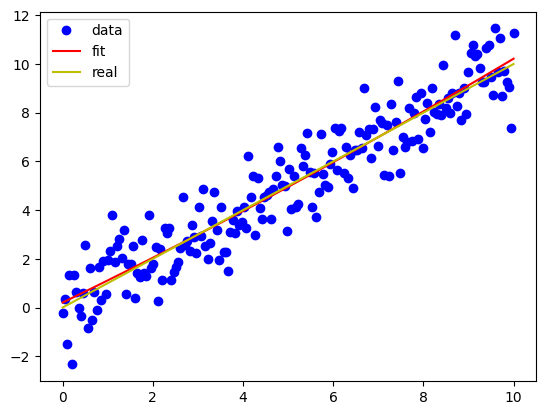
\includegraphics[width=0.5\textwidth]{Immagini/esempi/retta.png}
    \centering
    \label{fig:retta_fit}
\end{figure}
\subsection{Approssimare una somma di seni}
Vediamo adesso l'approssimazione di una figura più complessa.
Procediamo a dichiarare la base e generare i dati come mostrato nel listato \ref{gen_seni}.

\begin{lstlisting}[language=Python, caption={Generazione somma di seni},label=gen_seni]
    base  = B_Spline(
        knots=np.linspace(0,10,30+1),
        order=3
    )
    
    hb = HB_Spline(base)
        
    samples = np.shape(
        base.compute_base().get_collocation_matrix()
    )[1]
    
    x = np.linspace(0, 10, samples)
    y_real = np.sin(x) + np.sin(2 * x) + np.sin(3 * x)
    y = y_real + np.random.normal(0, 1, samples)
    
    data = np.matrix([x, y]).T
\end{lstlisting}
Eseguendo il codice mostrato nel listato \ref{fit_seno}, otteniamo il grafico di output mostrato nella figura a sinistra 
della tabella \ref{tab:seno_fit}.
\begin{lstlisting}[language=Python, caption={Fit somma di seni},label=fit_seno]
    model = Model(
        base=hb,
        data=data
    ).fit()
    
    model.plot()
    plt.plot(x, y_real, "y-", label="real")
    plt.legend(loc="best")
\end{lstlisting}

Dalla figura a sinistra in tabella \ref{tab:seno_fit}, possiamo notare che nell'intervallo $(2,4)$ non c'è un buon adattamento. Tuttavia se proviamo a 
a raffinare, otteniamo un risultato peggiore. Eseguendo il listato \ref{seno_overfitting} otteniamo la 
figura a destra in tabella \ref{tab:seno_fit}

\begin{lstlisting}[language=Python, caption={Overfitting nella somma di seni},label=seno_overfitting]
    model.refine((2,4))
    model.plot()
    plt.plot(x, y_real, "y-", label="real")
    plt.legend(loc="best")   
\end{lstlisting}

\begin{table}
    \centering
    \caption{Fit della funzione $sin(2x) + sin(3x) + \varepsilon$. \\ Overfitting nella figura a destra in $(2,4)$.\label{tab:seno_fit}}
        \begin{tabular}{ccc}
             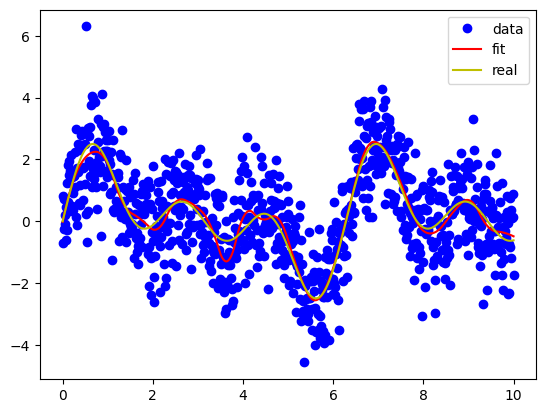
\includegraphics[width=0.45\linewidth]{Immagini/esempi/somma_seni.png}
            & 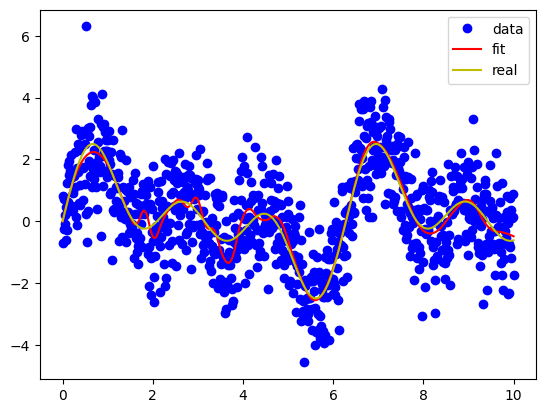
\includegraphics[width=0.45\linewidth]{Immagini/esempi/seno_overfit.png}\\[-4pt]
        \end{tabular}%
\end{table}

\begin{remark}
    La curva che è in overfitting  figura a sinistra della tabella \ref{tab:seno_fit} ha un \textbf{MSE} più basso rispetto 
    alla curva che non è in overfitting ,visibile nella figura a destra della tabella \ref{tab:seno_fit}, 
    infatti si ha un migliore adattamento ai dati, 
    che però sono rumorosi, e ci si allontana dalla vera funzione generatrice $sin(2x) + sin(3x)$. 
    I due MSE sono riportati in tabella \ref{tab:seno_mse}.

    \begin{table}[h!]
        \centering
        \caption{MSE per la funzione $sin(2x) + sin(3x)$, tab \ref{tab:seno_fit}}\label{tab:seno_mse}
         \begin{tabular}{||c c ||} 
         \hline
         Overfitting & Non Overfitting \\ [0.5ex] 
         \hline\hline
         1.0197649870617647 & 1.027356972130468 \\  [1ex] 
         \hline
         \end{tabular}
        \end{table}
\end{remark}

\subsection{La funzione di Runge}
Abbiamo scelto di approssiamare la funzione di Runge per vedere se si presenta il fenomeno di Runge.
\begin{definition}[Fenomeno di Runge]
    Il fenomeno di Runge è un problema relativo all'interpolazione polinomiale su nodi equispaziati con polinomi di grado elevato. 
    Esso consiste nell'aumento di ampiezza dell'errore in prossimità degli estremi dell'intervallo.
\end{definition}
Nel nostro caso abbiamo nodi equidistanti, ma grado basso. Non ci aspettiamo il verificarsi di tale fenomeno.

Mostraimo adesso i plot delle approssimazioni di tale funzione con rifinitura a mano negli intervalli $(-0.25,0.25)$ e successivamente 
in $(-0.1,0.1)$ e con rifinutura automatica basandosi su MSE per la scelta degli intervalli da rifinire. I risultati sono mostrati nella 
tabella \ref{tab:runge_fit}.
In tabella \ref{tab:runge_mse} sono rappresentati gli MSE per entrambe le versioni. Con il metodo manuale si ottiene un MSE minore 
e un maggior adattamento visivo alla vera curva.

\begin{table}
    \centering
    \caption{Rifinitura automatica(sinistra). Rifinitura manuale(destra)\label{tab:runge_fit}}
        \begin{tabular}{ccc}
             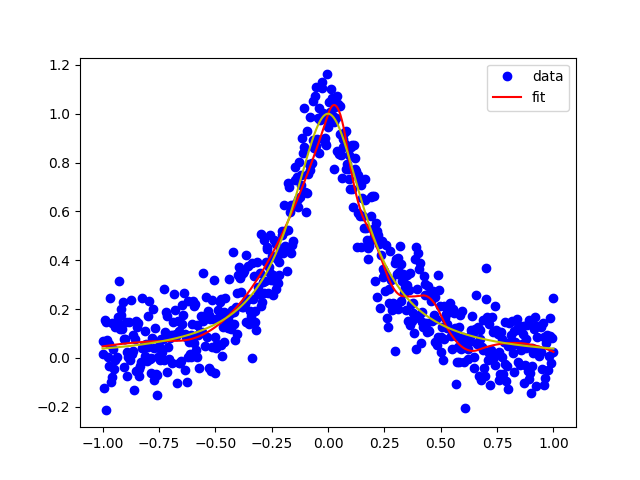
\includegraphics[width=0.45\linewidth]{Immagini/esempi/runge_auto.png}
            & 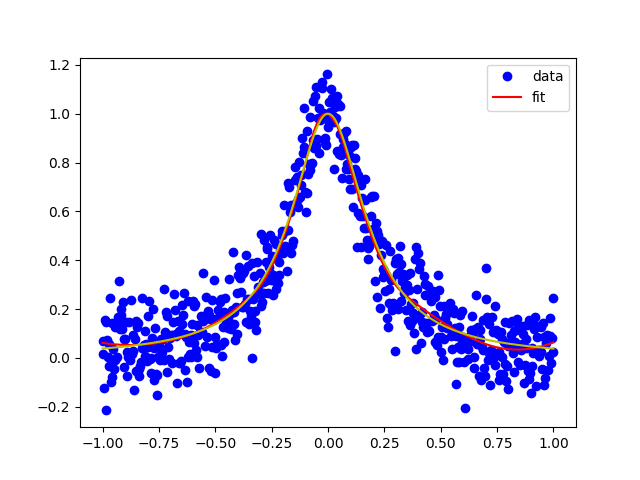
\includegraphics[width=0.45\linewidth]{Immagini/esempi/runge_mano.png}\\[-4pt]
        \end{tabular}%
\end{table}

\begin{table}[h!]
    \centering
    \caption{MSE per l'approssimazione della funzione di Runge}\label{tab:runge_mse}
     \begin{tabular}{||c c ||} 
     \hline
     Automatico & Manuale \\ [0.5ex] 
     \hline\hline
     0.010646661450860125 & 0.00981932028930905 \\  [1ex] 
     \hline
     \end{tabular}
    \end{table}

\end{document}